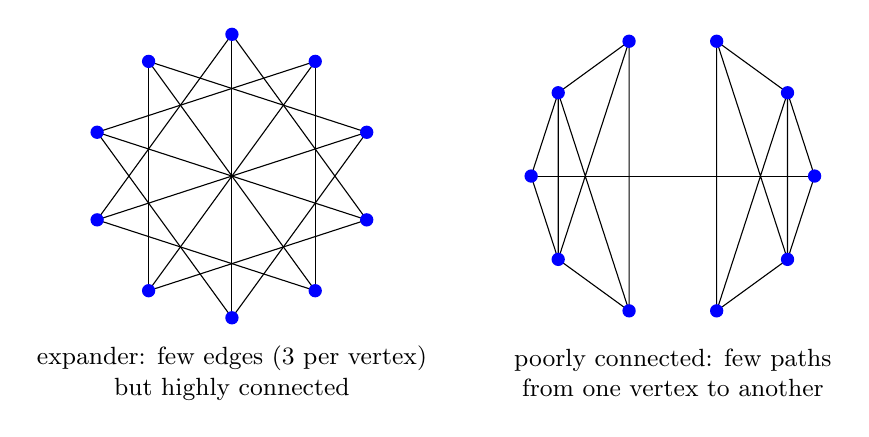
\begin{tikzpicture}[font=\small, vtx/.style={circle, fill=blue, inner sep=1.7pt}]
% ---------- an expander-like 3-regular graph on 10 vertices ----------
\begin{scope}
  \foreach \i in {0,...,9} \coordinate (u\i) at ({90+36*\i}:1.8);
  \foreach \i in {0,...,9} {
    \pgfmathtruncatemacro{\j}{mod(\i+3,10)}
    \draw (u\i) -- (u\j);
  }
  \foreach \i in {0,...,4} {
    \pgfmathtruncatemacro{\j}{\i+5}
    \draw (u\i) -- (u\j);
  }
  \foreach \i in {0,...,9} \node[vtx] at (u\i) {};
  \node[align=center] at (0,-2.5) {expander: few edges (3 per vertex)\\but highly connected};
\end{scope}
% ---------- a poorly connected graph: two clusters joined by one edge ----------
\begin{scope}[xshift=5.6cm]
  \foreach \i/\a in {1/108, 2/144, 3/180, 4/216, 5/252} {
    \coordinate (l\i) at (\a:1.8);
    \coordinate (r\i) at ({180-\a}:1.8);
  }
  \foreach \s in {l, r} {
    \draw (\s1) -- (\s2) (\s1) -- (\s4) (\s1) -- (\s5) (\s2) -- (\s4) (\s2) -- (\s5) (\s4) -- (\s5)
          (\s3) -- (\s2) (\s3) -- (\s4);
  }
  \draw (l3) -- (r3);
  \foreach \i in {1,...,5} { \node[vtx] at (l\i) {}; \node[vtx] at (r\i) {}; }
  \node[align=center] at (0,-2.5) {poorly connected: few paths\\from one vertex to another};
\end{scope}
\end{tikzpicture}
